\documentclass{article}
\usepackage{graphicx}
\usepackage[margin=1.2in]{geometry}
\graphicspath{ {../Results/} } \usepackage{caption}

\begin{document}

\title{High Performance Computing (HPC) Practical{}}
\author{Jacob Griffiths}

\maketitle

\section*{Neutral Theory}

\bigskip

\subsection*{Question 8}
Despite no species having superior fitness in a neutral model, 
the system will always converge to monodominance
as time elapses if speciation is not incorporated. This is because as a species becomes more
numerous by chance, they now have a higher probability of 
being selected by the model to replace the removed individual at
the next neutral step. This advantage will perpetuate until only 
one species remains.

\begin{center}
    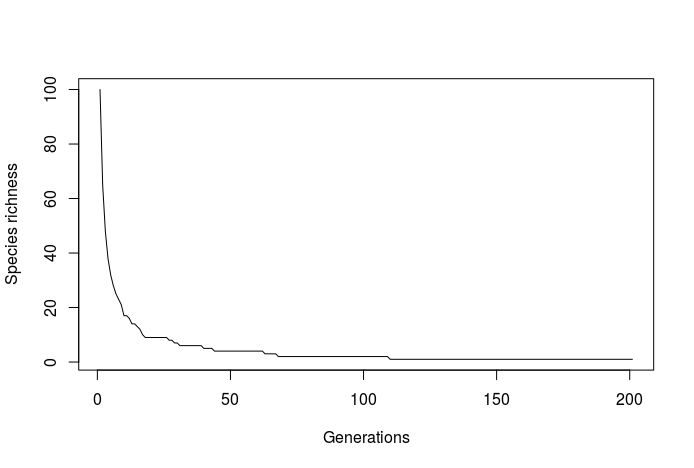
\includegraphics[width=\textwidth]{../Results/question_8.jpeg}
    \captionof{figure} {A neutral model simulation with a starting species
    richness of 100, modelled over 200 generations. The number of generations simulated
    is always half the starting community size}
\end{center}


\subsection*{Question 12}
This simulation compared the effect of different species richness
in starting communities and whether this affected the simulation.
Figure 2 clearly shows that despite one simulation starting with a 
species richness of 100 and the other with a richness of 1, they both 
ultimately converge at the same dynamic equilibrium with a richness
of approximately 25, after about 25 generations. This illustrates 
the importance of burn-in time during neutral theory simulations
by removing the effect of arbitrary starting values. It is worth noting
that these communities do not become monodominant as speciation has been 
incorporated into this model.

\begin{center}
  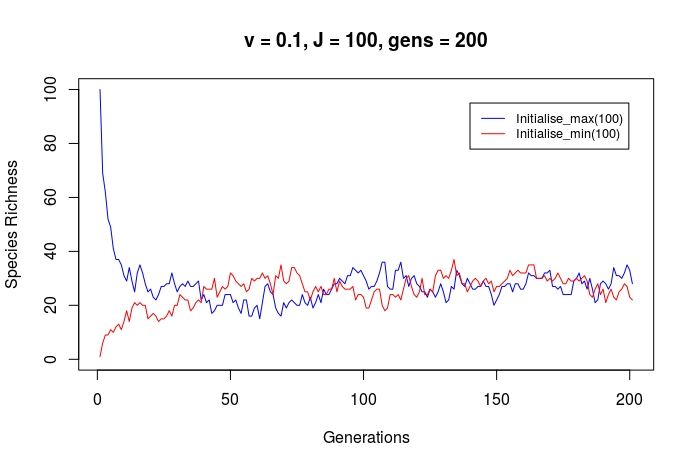
\includegraphics[width=\textwidth]{../Results/question_12.jpeg}
  \captionof{figure} {Comparison of different starting community species
  richness on neutral simulations. Initialise\_max(100) creates a community with
  species richness 100 and Initialise\_min(100) creates a community with species
  richness 1. A speciation rate (v) of 0.1 was used}
\end{center}

\break

\subsection*{Question 16}
This simulation ran a neutral model for a burn-in time of 
200 generations before recording species abundance octaves
every 20 generations for a further 2000 generations. Figure 
3 shows the starting community species richness has no effect
on the simulation if an adequate burn-in time is used.

\begin{center}
  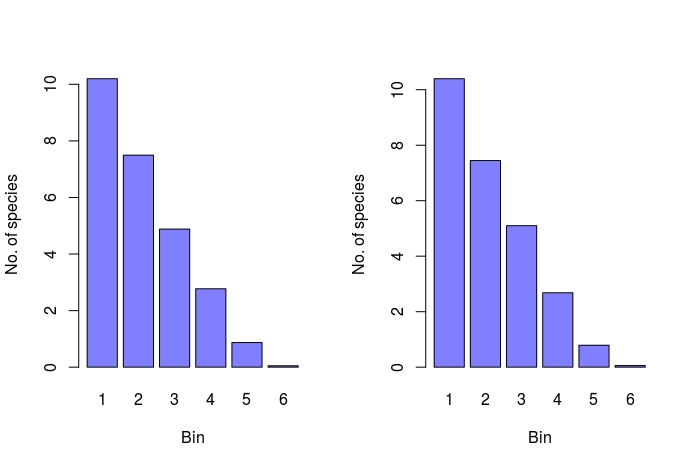
\includegraphics[width=\textwidth]{../Results/question_16.jpeg}
  \captionof{figure} {Number of species in each 'octave class' for two neutral
  simulations. Left is a community that started with species richness 100 and right
  is a community that started with species richness 1. The speciation rate was 0.1.}
\end{center}

\break

\subsection*{Challenge Question A}
As found previously, starting community richness has no impact on the richness once
dynamic equilibrium is reached. In this simulation it took approximately 2000 neutral
steps to reach equilibrium.

\begin{center}
  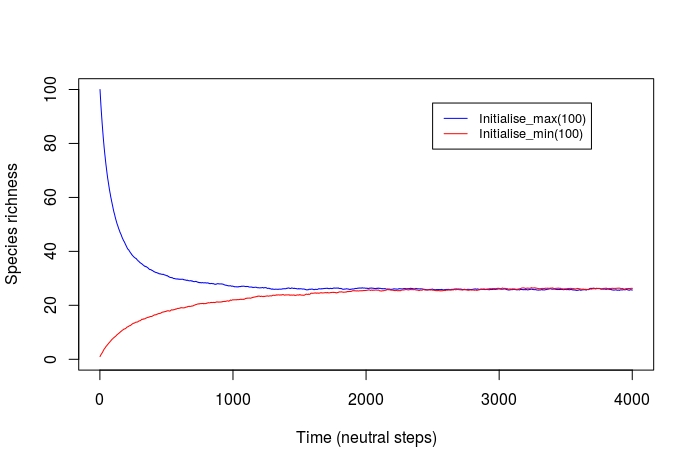
\includegraphics[width=\textwidth]{../Results/challenge_A.jpeg}
  \captionof{figure} {Species richness of two different starting communities over
  4000 neutral steps and averaged across 200 simulations. A speciation rate of 0.1 was
  used.}
\end{center}

\subsection*{Challenge Question B}

\begin{center}
  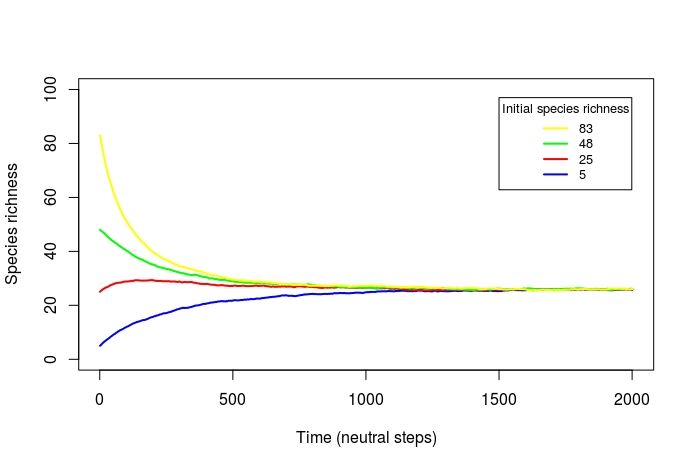
\includegraphics[width=\textwidth]{../Results/challenge_B.jpeg}
  \captionof{figure} {Species richness over time with four different initial 
  community species richnesses. The same speciation rate was used as in Figure 4
  and clearly all communities converge on the same dynamic equilibrium regardless 
  of initial species richness}
\end{center}

\subsection*{Question 20}

\begin{center}
  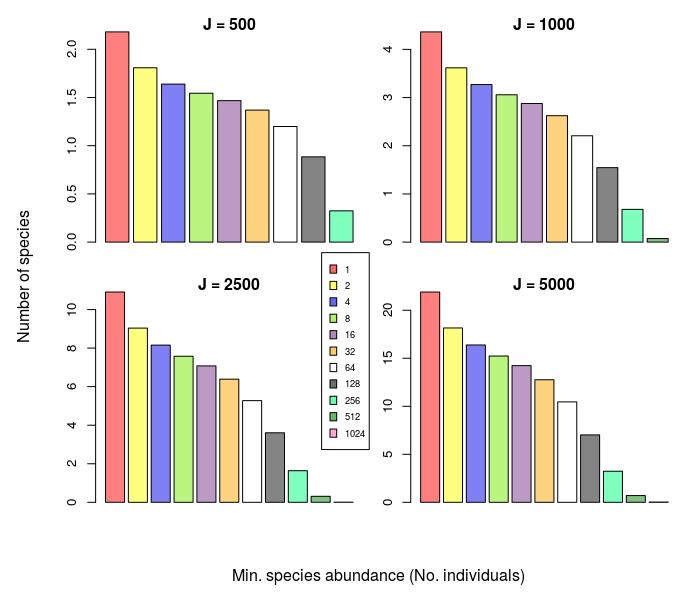
\includegraphics[width=\textwidth]{../Results/question_20.jpeg}
  \captionof{figure} {Average octave classes over 25 simulations in each community size (J).
  All simulations were run using high-performance computing for 12 hours. A burn-in time of 
  J/10 generations was used and not incorporated in these averages. Each octave class doubles 
  in abundance as you move one to the right.}
\end{center}

\subsection*{Challenge Question C}

\begin{center}
  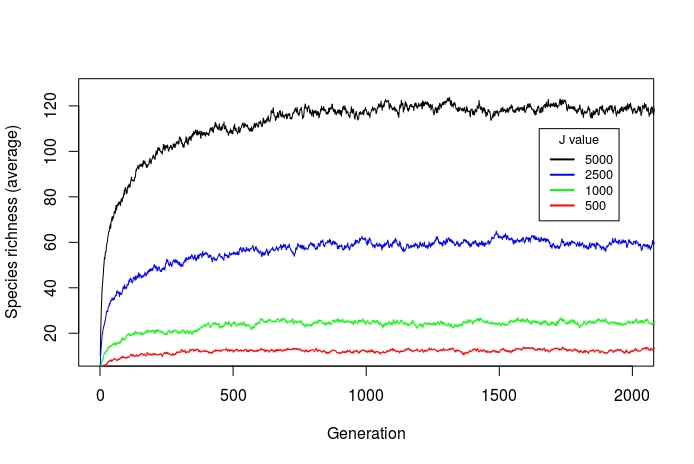
\includegraphics[width=\textwidth]{../Results/challenge_C.jpeg}
  \captionof{figure} {Mean species richness over 2000 generations of the HPC simulations.
  Community size clearly affects the mean species richness and the larger communities take more
  generations to reach dynamic equilibrium}
\end{center}

\bigskip

\subsection*{Challenge Question D}
Further simulations were carried out on the system using coalescence. This alternative method
was used to verify the results from the HPC simulations. Both methods produced the same results 
but the coalescence method was significantly faster despite running a lot more simulations for each 
community size (J=500 took 16.45s, J=1000 took 35s, J=2500 took 123s, and J=5000 took 357s, compared with
11.5 hours for every simulation with HPC). As 
coalescence works backwards from a starting community, it only computes the necessary steps to calculate
the present species richness and abundance and doesn't waste time simulating species that previously became extinct.
The HPC simulations, however, started at a theoretical point in the past and worked forward, wasting 
significant CPU time simulating species that became extinct. However, coalescence isn't as good for time-series
simulations and does not incorporate additional parameters as easily

\break

\section*{Fractals in Nature} 

\bigskip

\subsection*{Question 21}
Fractals are defined as objects that have a non-integer number 
of dimensions. Therefore, a line (dimension=1), a square (dimension=2)
and a cube (dimension=3) are not fractals. To calculate the dimension
of a fractal the following formula is required:
\[ size = width^{dimension} \]
Where width is the width of the fractal at that level and size is the number of subunits
that make up that level of the fractal. This can be log-transformed and
rearranged for dimension:
\[ dimension = log(size)/log(width) \]
Applying this formula to the question provided returns the dimension of object
1 (left of page) as 1.893 and the dimension of object 2 (right of page) as 2.727.

\bigskip

\subsection*{Question 22}
The chaos\_game function drew a Sierpinski Gasket (Figure 8) on a plot in R. As the number of 
repeats increased, the edges became denser so the object becomes more 
and more well-defined.

\begin{center}
  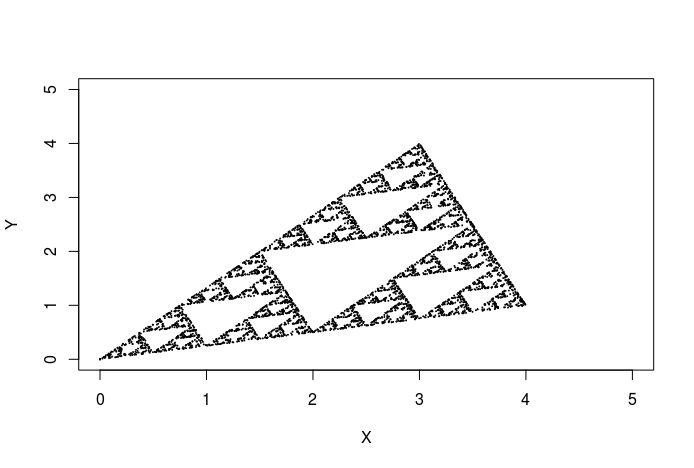
\includegraphics[width=\textwidth]{../Results/question_22.jpeg}
  \captionof{figure} {The Sierpinski Gasket as plotted by the chaos game function.}
\end{center}

\subsection*{Challenge question E}
In this exercise the starting point (X) and the distance divisor (2 used before) were varied to explore
their effects on the resulting plot. Figure 4 demonstrates that variation in X has
little effect on the plot as points are plotted towards the triangle and once there, 
the behaviour continues as before. Varying the divisor had a far greater effect. The Gasket 
immediately broke down as it was increased and the points seemed to be becoming closer and closer 
to a straight line leading from X. This makes sense as no matter how small the divisor,
you'd still expect the points to reach the center of ABC eventually but once there 

\begin{center}
  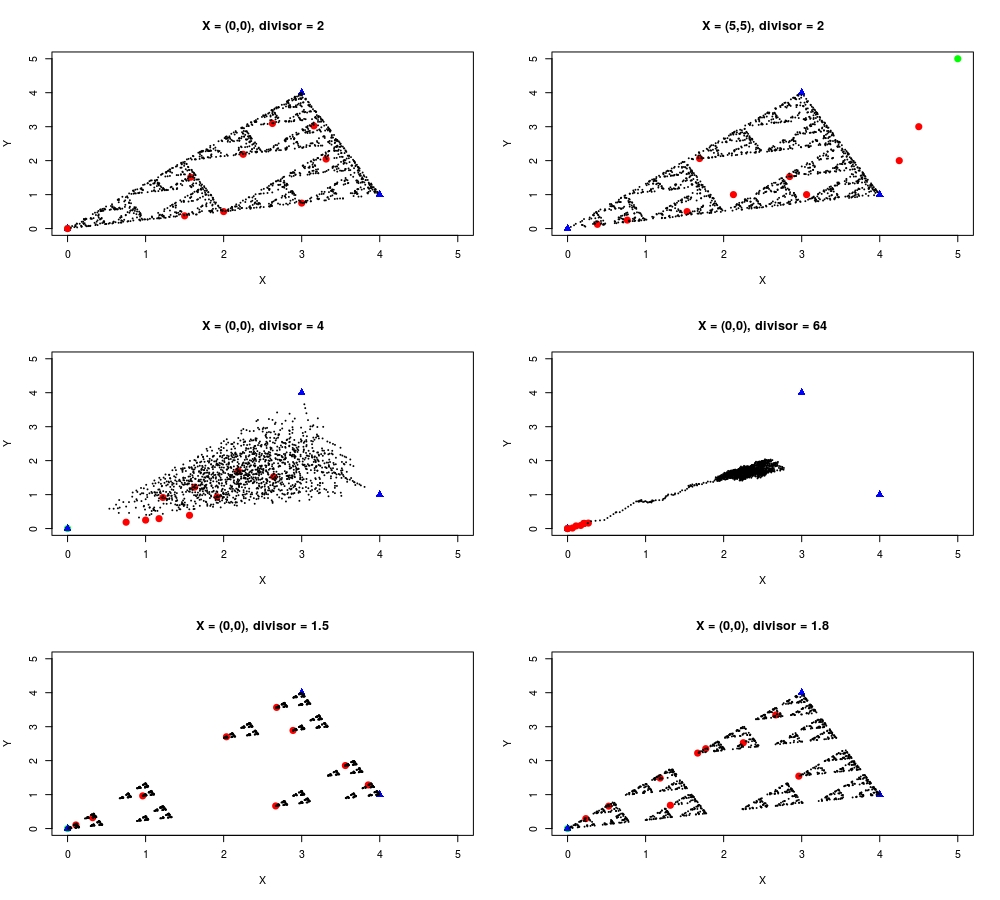
\includegraphics[width=\textwidth]{../Results/challenge_E.jpeg}
  \captionof{figure} {Sierpinski Gasket with a variety of X values and divisors. Changing X has no effect
  on the Gasket but the divisor does. Green points indicate the X start point, red points indicate 
  the first 10 points of X, and the blue triangles indicate the values of A, B, and C that were used as the 
  points of the Gasket. Increasing the divisor causes the Gasket to break down but decreasing it causes several
  smaller Gaskets to form.}
\end{center}

\break

\subsection*{Question 25}
The 'spiral' function draws a line between two points by calling the 'turtle'
function then calls itself iteratively to draw a spiral. This does work to some extent but 
eventually R stops the function and returns an error due to the infinite recursion.
\bigskip

\subsection*{Question 26}

\begin{center}
  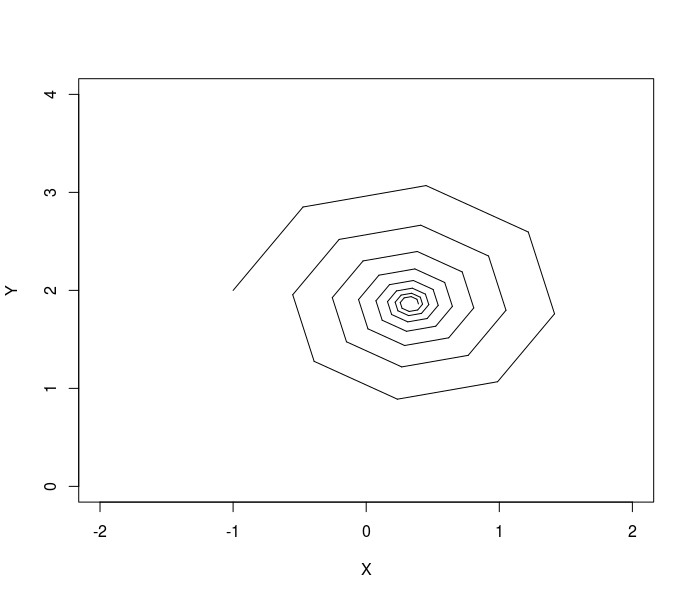
\includegraphics[width=\textwidth]{../Results/question_26.jpeg}
  \captionof{figure} {The output of the 'spiral\_2' function using a starting point of 
  (-1,2), an angle of 45 degrees and a starting line length of 1. The infinite recursion of
  'spiral' was avoided in this function by terminating the function when the line length got
  to a specified size}
\end{center}

\subsection*{Question 27}
\begin{center}
  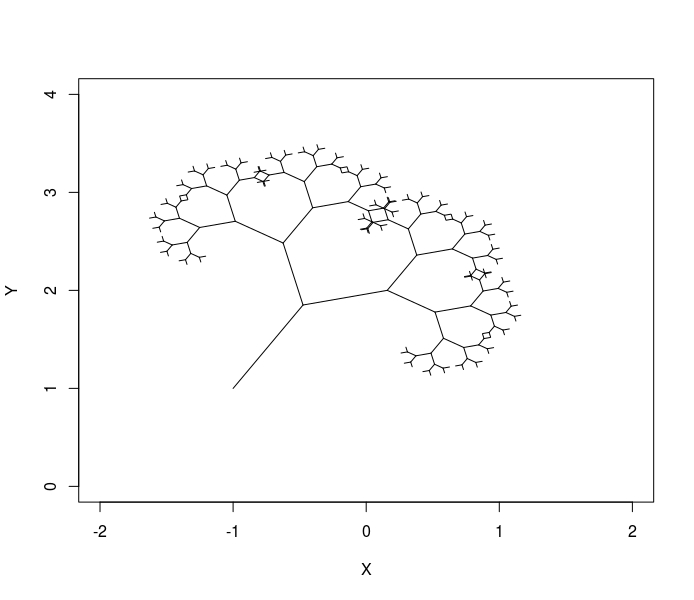
\includegraphics[width=\textwidth]{../Results/question_27.jpeg}
  \captionof{figure} {An extension of the 'spiral\_2' function called 'tree'.
  It calls itself twice, once for left and once for right at the same angle
  to make this tree-like structure.}
\end{center}

\subsection*{Question 29}
\begin{center}
  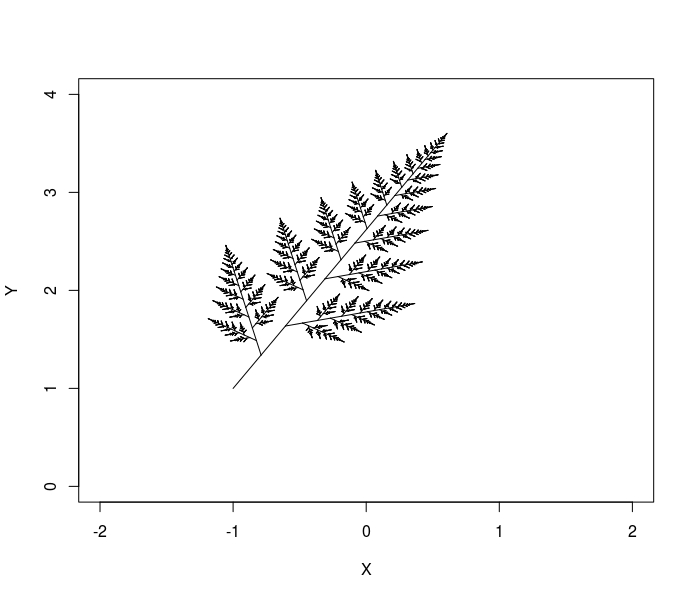
\includegraphics[width=\textwidth]{../Results/question_29.jpeg}
  \captionof{figure} {An extension of the 'tree' function that either calls itself
  and goes left or right, or goes straight on. The code ensure that the direction always
  alternates, creating this fern-like structure.}
\end{center}

\subsection*{Challenge Question F}
\begin{center}
  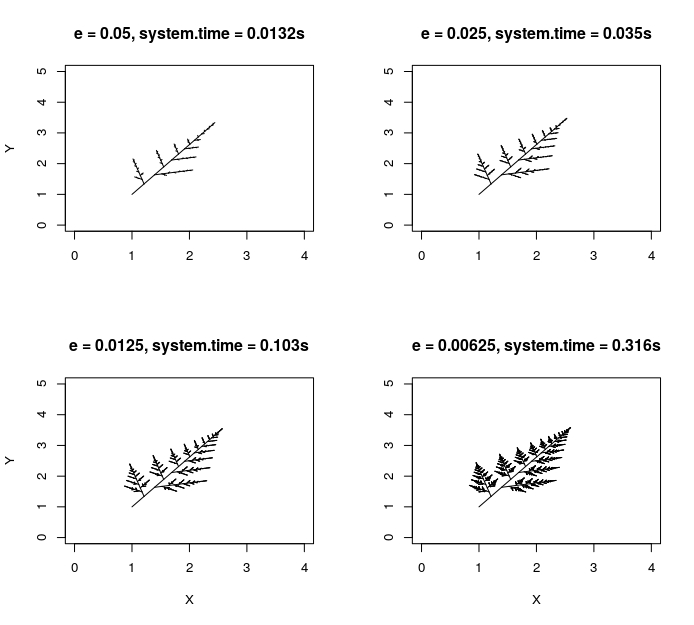
\includegraphics[width=\textwidth]{../Results/challenge_F.jpeg}
  \captionof{figure} {Varying the input parameter 'e' in the 'fern\_2' function to see
  its effect. 'e' determines the line length that the function will stop looping at so a lower
  'e' value will give a more detailed plot that takes longer to run as can be seen here.}
\end{center}


\end{document}